\section{Web-based Disease Surveillance}

Early and timely detection of disease outbreaks ushered the rise of newer technologies that could augment existing systems of disease surveillance \cite{chunara2012new}. Web-based technologies in particular have been shown to provide ``greater communication and improved surveillance and reporting frameworks,'' improving the timeliness of outbreak detection \cite{chan2010global}. Such surveillance systems are also ``intuitive, adaptable, low-cost, and [operate] in real-time'' \cite{choi2016web}, ``with reduced cost and increased reporting transparency'' \cite{wilson2009early}. This demonstrates the advantages of using such approaches in disease detection. 

A study by Choi \textit{et al.} lists down several web-based technologies that have been employed for identifying emerging infectious diseases, shown in Figure \ref{fig:webbased} \cite{choi2016web}. Most of these systems utilize text mining social media posts and news reports online \cite{brownstein2009digital}. 

\begin{figure}[t]
    \centering
    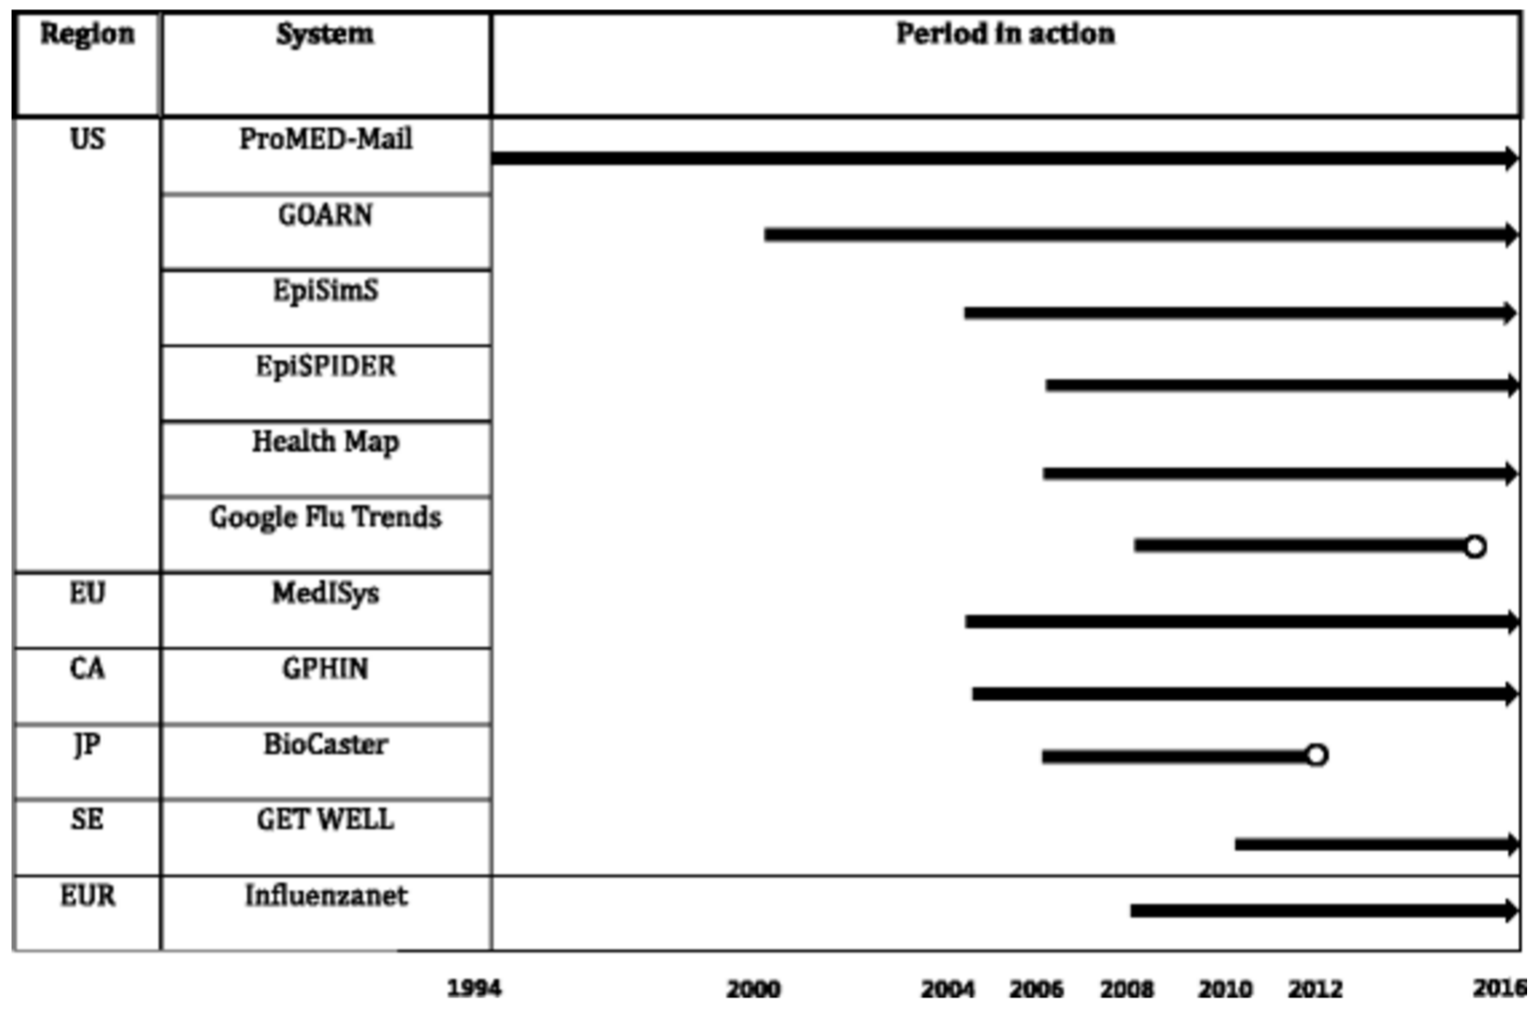
\includegraphics[width=\textwidth]{WebBasedSurveillance}
	\caption{Development of web-based surveillance systems in chronological order \cite{choi2016web}.}
	\label{fig:webbased}
\end{figure}

It has been shown that tweets can be useful in retrieving health-related information generated by users. One study demonstrated an algorithm that can capture tweets and classify them to ascertain if they are ``infodemiological'' (and can be epidemiological purposes) or otherwise \cite{espina2016towards}. Another study presented a topic model for Twitter ``that associates symptoms, treatments and general words with diseases'' \cite{paul2012model}. Both concluded that it is feasible to extract health information from tweets. Multiple studies have also implemented mining health information from tweets, concluding that crowd-source social media-based monitoring tools can provide ``timely information about the state of an epidemic'' \cite{lampos2010tracking, boulos2011crowdsourcing}.

User-generated health information could lead to more expedient recognition of public health events \cite{velasco2014social} through this rapid generation of information, faster than collection of health information from individual health workers in traditional surveillance systems.

Other sources of unstructured information such as Internet news sites have been shown to be relevant in providing ``detailed local and near-real time data on disease outbreaks'' \cite{heymann2001hot,madoff2005internet,morse2007global}. As such, news sites have been used by event-based global surveillance systems such as Global Public Health Intelligence Network (GPHIN), HealthMap, and EpiSPIDER \cite{keller2009use}. The aforementioned systems acquire news articles through Really Simple Syndication (RSS) feeds, news aggregators and news wires, electronic mailing lists, and web scraping techniques. These systems then subject gathered articles to clustering, linguistic analysis, and cross-referencing with other sources to determine their accuracy and relevance \cite{keller2009use}. 

Moderated reporting and information dissemination systems such as the Program for Monitoring Emerging Diseases (ProMED-Mail) and Global Outbreak Alert Response Network (GOARN) also integrate news sites to facilitate networked discussion towards an ``international coordinated response to outbreaks'' \cite{choi2016web}.
